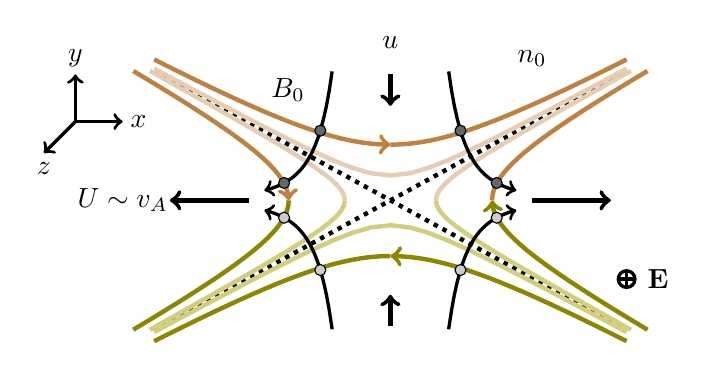
\begin{tikzpicture}[scale=1.0]

%\newcommand\XA{2} etc. and then \coordinate (A) at (\XA,\YA);

%\tikzset{declare function={f(\x)=\x;}}

\def\Xmin{-3.0}
\def\Xmax{+3.0}

\def\Ome{0.3}
\def\Lia{0.5}
\def\Lib{0.3}
\def\Lic{0.1}

\draw [domain=\Xmin: \Xmax, ultra thick, dotted] plot(\x,{-sqrt(\Ome)*\x});
\draw [domain=\Xmin: \Xmax, ultra thick, dotted] plot(\x,{ sqrt(\Ome)*\x});

\draw [domain=\Xmin: 0, ultra thick, draw=brown, ->] plot(\x,{sqrt( \Ome*\x*\x+\Lia)});
\draw [domain=0: \Xmax, ultra thick, draw=brown] plot(\x,{sqrt( \Ome*\x*\x+\Lia)});
\draw [domain=\Xmin: \Xmax, ultra thick, draw=brown!40] plot(\x,{sqrt( \Ome*\x*\x+\Lic)});

\draw [domain=\Xmin: 0, ultra thick, draw=olive] plot(\x,{-sqrt( \Ome*\x*\x+\Lia)});
\draw [domain=0: \Xmax, ultra thick, draw=olive, <-] plot(\x,{-sqrt( \Ome*\x*\x+\Lia)});
\draw [domain=\Xmin: \Xmax, ultra thick, draw=olive!40] plot(\x,{-sqrt( \Ome*\x*\x+\Lic)});

\draw [domain=\Xmin*sqrt(\Ome): 0, ultra thick, draw=olive, ->] plot({sqrt((\x*\x+\Lia)/\Ome)}, \x);
\draw [domain=0: \Xmax*sqrt(\Ome), ultra thick, draw=brown] plot({sqrt((\x*\x+\Lia)/\Ome)}, \x);
\draw [domain=\Xmin*sqrt(\Ome): 0, ultra thick, draw=olive!40] plot({sqrt((\x*\x+\Lic)/\Ome)}, \x);
\draw [domain=0: \Xmax*sqrt(\Ome), ultra thick, draw=brown!40] plot({sqrt((\x*\x+\Lic)/\Ome)}, \x);

\draw [domain=\Xmin*sqrt(\Ome): 0, ultra thick, draw=olive] plot({-sqrt((\x*\x+\Lia)/\Ome)}, \x);
\draw [domain=0: \Xmax*sqrt(\Ome), ultra thick, draw=brown, <-] plot({-sqrt((\x*\x+\Lia)/\Ome)}, \x);
\draw [domain=\Xmin*sqrt(\Ome): 0, ultra thick, draw=olive!40] plot({-sqrt((\x*\x+\Lic)/\Ome)}, \x);
\draw [domain=0: \Xmax*sqrt(\Ome), ultra thick, draw=brown!40] plot({-sqrt((\x*\x+\Lic)/\Ome)}, \x);

\def\KKK{0.6}
\def\XmiN{-1.6}
\def\XmaX{-0.74}

\draw [domain=\XmaX: \XmiN, very thick, ->] plot(\x, {\KKK*(-\x)^(-1/\Ome)});
\draw [domain=\XmaX: \XmiN, very thick, ->] plot(\x, {-\KKK*(-\x)^(-1/\Ome)});
\draw [domain=-\XmaX: -\XmiN, very thick, ->] plot(\x, {\KKK*(\x)^(-1/\Ome)});
\draw [domain=-\XmaX: -\XmiN, very thick, ->] plot(\x, {-\KKK*(\x)^(-1/\Ome)});


\def\Xa{0.89}
\def\Xb{1.35}

\filldraw[fill=black!60] (\Xa, {\KKK*(\Xa)^(-1/\Ome)}) circle (2pt);
\filldraw[fill=black!60] (\Xb, {\KKK*(\Xb)^(-1/\Ome)}) circle (2pt);
\filldraw[fill=black!60] (-\Xa, {\KKK*(\Xa)^(-1/\Ome)}) circle (2pt);
\filldraw[fill=black!60] (-\Xb, {\KKK*(\Xb)^(-1/\Ome)}) circle (2pt);

\filldraw[fill=black!20] (\Xa, -{\KKK*(\Xa)^(-1/\Ome)}) circle (2pt);
\filldraw[fill=black!20] (\Xb, -{\KKK*(\Xb)^(-1/\Ome)}) circle (2pt);
\filldraw[fill=black!20] (-\Xa, -{\KKK*(\Xa)^(-1/\Ome)}) circle (2pt);
\filldraw[fill=black!20] (-\Xb, -{\KKK*(\Xb)^(-1/\Ome)}) circle (2pt);



\draw[very thick] ( 3.0,-1.0) circle (3pt);
\draw[very thick] ( 2.9,-1.0) -- ( 3.1,-1.0);
\draw[very thick] ( 3.0,-1.1) -- ( 3.0,-0.9);
\node at ( 3.4,-1.0) {$\mathbf E$};

\draw[ultra thick, <-] (-2.8, 0) -- (-1.8, 0);
\draw[ultra thick, ->] (1.8, 0) -- (2.8, 0);
\node at (-3.4, 0.0) {$U \sim v_A$};

\draw[ultra thick, ->] ( 0.0, 1.6) -- ( 0.0, 1.2);
\draw[ultra thick, <-] ( 0.0,-1.2) -- ( 0.0,-1.6);
\node at ( 0.0, 2.0) {$u$};

\node at (-1.3, 1.4) {$B_0$};
\node at ( 1.8, 1.8) {$n_0$};


\draw[very thick, ->] (-4.0, 1.0) -- (-3.4, 1.0);
\node at (-3.2, 1.0) {$x$};
\draw[very thick, ->] (-4.0, 1.0) -- (-4.0, 1.6);
\node at (-4.0, 1.8) {$y$};
\draw[very thick, ->] (-4.0, 1.0) -- (-4.4, 0.6);
\node at (-4.4, 0.4) {$z$};


\end{tikzpicture}
